\newpage
\section{Firmware engineering - Chloe }
\label{sec:fw}


\subsection{Firmware architecture}

\begin{figure}[ht]
    \centering
    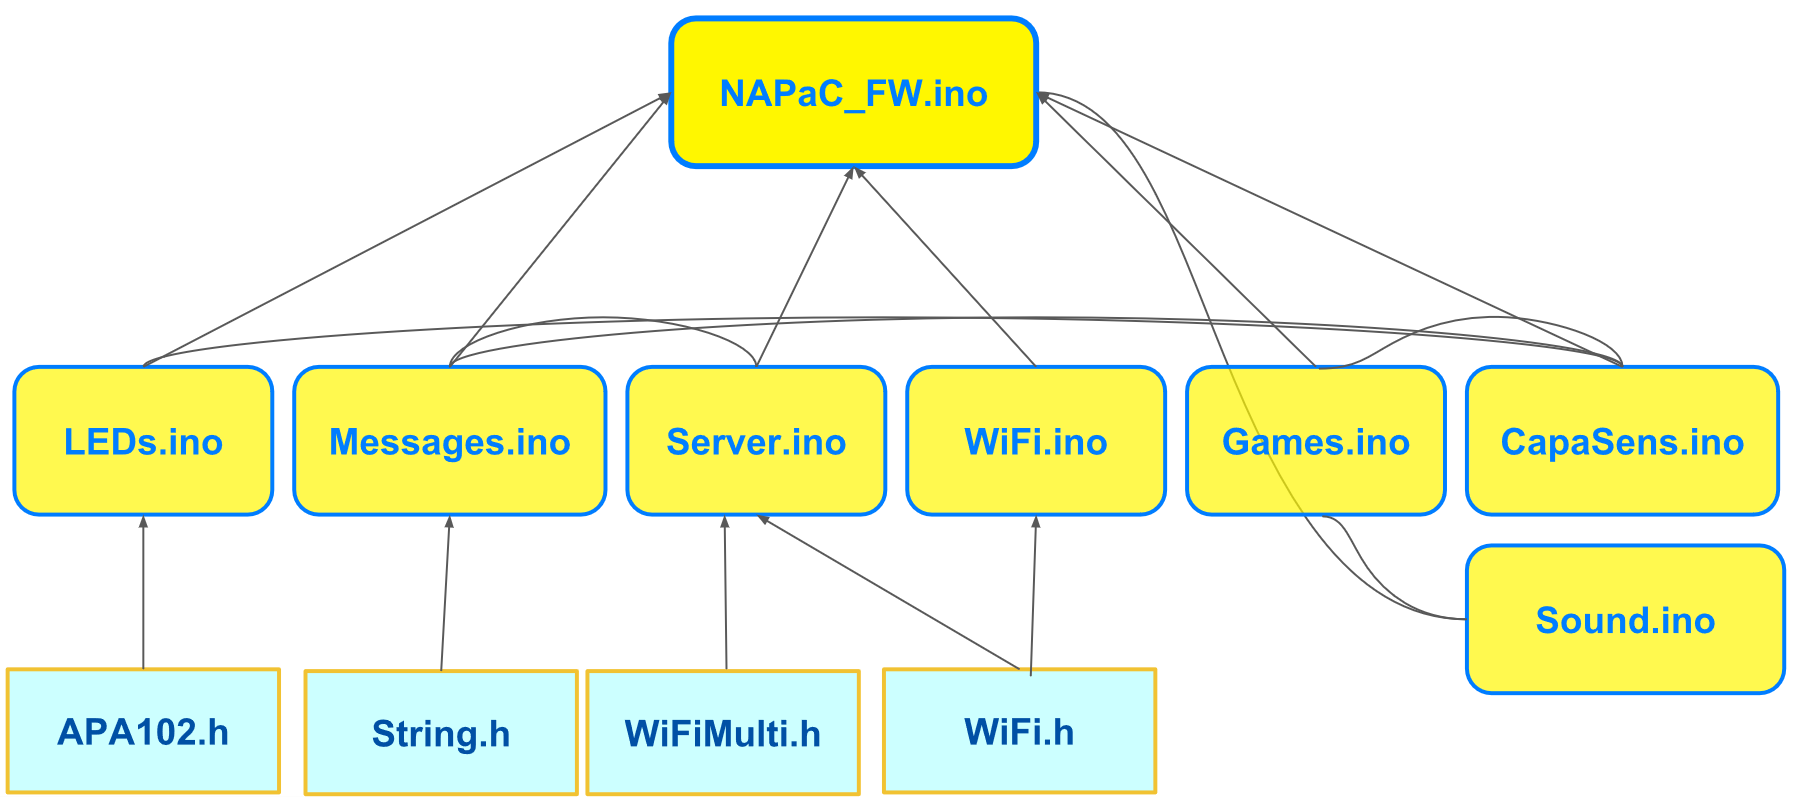
\includegraphics[width=\textwidth]{images/FW/FW_architecture.PNG}
    \caption{Firmware architecture diagram with units and libraries}
    \label{fig:FW_architecture}
\end{figure}

The chosen architecture for our Arduino program is illustrated in Figure \ref{fig:FW_architecture}. The main file (NAPaC\_FW.ino) calls each separate unit which may call eachother depending on the implemented functions.
Each unit is conceived as a "library", with its setup function and functions relative to a hardware component or interaction.

\begin{description}[align=left]
\item  [NAPaC\_FW.ino] Used as the main file for our firmware. Runs through setup functions for each unit then calls the other functions (game interaction) from the loop. 
\item [LEDs.ino] Based on the APA102 library, this unit defines LED pins and sets up LED strips and output pins during setup. In this unit, we define principal actions for LEDs such as turning on in defined colour, blinking, and turning on the LEDs in appropriate colours according to the game steps defined in figure \ref{fig:game_diagram}.
\item[Messages.ino] This unit defines the "alphabet" in accordance with the communication protocol defined in Table \ref{tab:comm_message}. This unit also holds functions for sending defined interaction messages to the server.
\item[Server.ino] The Server module had functions for connecting to the server, reading and sending messages as well as close server connection. 
\item[Games.ino] The Games unit is the main file for interactions. It has functions defining a solo game and the game with parents, and keeps record of the Zone status (off, on, colour) for the plush toy. It also has functions defining the beginning and end of game sessions which interact with the server to open and close games.
\item[CapaSens.ino] In this unit, we set up the capacitive touch sensors and define the touch status with the touch library provided by ESP32. 
\item[Sound.ino] The Sound unit enables the microcontroller to play sounds through the buzzer. We have defined the standard Western muscial scale (Do-Re-Mi-...) and implemented several sound tests and jingles for the games. 
\end{description}



    \subsubsection{Choice of coding environment}
After experimenting with both ESP32 Eclipse framework and the Arduino environment, we decided to chose Arduino as our coding platform for the widely available examples and ease of programming.
    \paragraph{Libraries}
In our project, we use libraries for the APA102 LEDs, WiFi configuration and capacitive touch sensors. Their main parameters and working principles are described below. 
    
\subsection{Description of Functions}

\subsubsection{NAPaC\_FW}

\paragraph{Setup}
The setup function runs through the induvidual setup functions of each unit: LEDs, Capacitive Sensors, Sound. It then proceeds to find WiFi SmartConfig (or connect to WiFi using an existing one), connects to server then sends a "presentation" message to the server sending its ID.

\lstinputlisting[style=Arduino, firstline=13, lastline=26]{code_snippets/arduino/NAPaC_FW.ino}

\paragraph{Main Loop}
In the main loop, the program waits for a message requesting the beginning of a game session. In a final version of the firmware we could expect functions such as checking for child's presence, sleep mode, etc. 

\lstinputlisting[style=Arduino, firstline=28]{code_snippets/arduino/NAPaC_FW.ino}

\subsubsection{Messages}
The messages unit is used to deal with sending messages to the server. These messages are defined in Section \ref{subsec:communication}. 

\paragraph{Alphabet setup}
This snippet of code sets up the characters required form the communication protocol. 
\lstinputlisting[style=Arduino, firstline=19, lastline=22]{code_snippets/arduino/Messages.ino}


\begin{description}[align=left]
\item[first\_message] The microcontroller sends a message to the server with its unique identifier, allowing the server to link it with its IP address.
\lstinputlisting[style=Arduino, firstline=35, lastline=39]{code_snippets/arduino/Messages.ino}
\item[accept\_game\_message] Sends the 2002 message meaning the child has accepted the parent's game request
\lstinputlisting[style=Arduino, firstline=42, lastline=47]{code_snippets/arduino/Messages.ino}
\item[LED\_on\_message] Sends message 2003 with LED ID of LED turned on by the child
\lstinputlisting[style=Arduino, firstline=50, lastline=57]{code_snippets/arduino/Messages.ino}
\item[LED\_off\_message] Sends message 2004 with LED ID of LED turned off by the child. This message is very similar to message 2003 above. 
%\lstinputlisting[style=Arduino, firstline=60, lastline=67]{code_snippets/arduino/Messages.ino}
\item[hello] Prints a welcoming message to serial.
\end{description}


\subsubsection{WiFi connectivity and Server communication}\label{subsec:fw/Functions/WiFi}
We use SmartConfig to send the WiFi configuration to the microcontroller from the parent's smartphone. The WiFi configuration can also be save to the program for easier programming. 
Our goal for China or next semester is to save a new SmartConfig to the EEPROM memory then retrieve it upon launch to connect to a known WiFi network. 
    
\paragraph{WiFi Smartconfig}
The Arduino SmartConfig libraries allow us to easily connect to a WiFi with configuration send by a nearby smartphone.
\lstinputlisting[style=Arduino, firstline=9, lastline=35]{code_snippets/arduino/WiFi.ino}

%The following function allows the microcontroller to connect to a hardcoded WiFi network. Our goal for China is to save a previously received configuration to the EEPROM, retrieve it then connect to the WiFi network using this configuration.  
%\lstinputlisting[style=Arduino, firstline=37, lastline=53]{code_snippets/arduino/WiFi.ino}


\paragraph{Connection to server}
The code below allows the microcontroller to connect to the server in order to enable communications with the parent's smartphone. 
\lstinputlisting[style=Arduino, firstline=7, lastline=31]{code_snippets/arduino/Server.ino}

\paragraph{Read message from server} This function reads a message sent by the parent's smartphone and transmitted through the server. It reads the message and saves it into a string that it returns. 
\lstinputlisting[style=Arduino, firstline=38, lastline=53]{code_snippets/arduino/Server.ino}

\subsubsection{Games}
The main part of our firmware and most visible to the user is the "game" interaction. For now, we have set one type of interaction, or one game, but could imagine implementing other ones. A solo game is also available for testing. Figure \ref{fig:game_diagram} presents the flowchart for the game interaction. The goal of the "game" is that either the parent or child can chose to turn on one or several LEDs which will also light up on the game partner's device. A sound corresponding to the zone will also be played. The LEDs turn on the colour of the player who turned them on and the other player can turn them off and then on in their colour. 

\begin{figure}[ht]
    \centering
    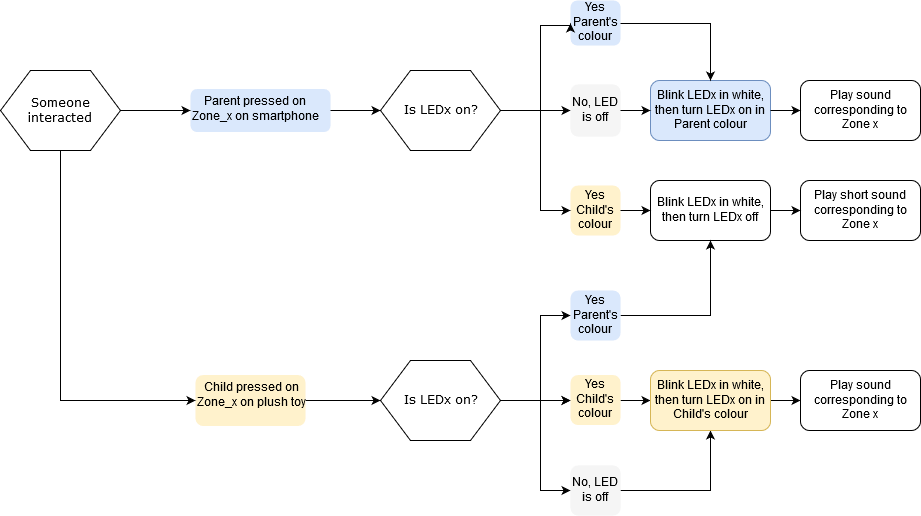
\includegraphics[width=\textwidth]{images/FW/FW_game_diagram.png}
    \caption{Flowchart for game interaction}
    \label{fig:game_diagram}
\end{figure}

\begin{description}[align=left]
\item
\end{description}

\subsubsection{Capacitive touch sensors}\label{sec:capa_sens}

The capacitive touch sensors are crucial for the child's interaction with the plush toy. The functions used in the firmware are listed below. In the prototype presented in MS5, we only distinguished between touched and untouched, but hope to find the right settings to have a better sensitivity to different kinds of touching or pressing through the skin and plush stuffing. 

\paragraph{CapaSens Functions} 

\begin{description}[align=left]
\item[setup\_capa] Sets up the capacitive touch sensor pins as inputs then reads the initial value of each touch sensor.
\item[touch\_read\_value(touch\_id)] Reads the value on sensor of given ID. 
\item[capa\_touched(touch\_id)] Returns PRESSED if the touch sensor is being touched or RELEASED if not. Further improvement would include different states of touch (touch, light press or strong press).
\item[presence] Returns 1 if any sensor is touched, meaning the child is holding or playing with the plush toy.
\item[test\_touch\_values] Test function which prints the sensor values in serial.
\item[test\_if\_touched] Test function printing in serial the ID and value of any touched sensor.
 \ldots  
\end{description}
    
\paragraph{Influence of sensing parameters}
The ESP32 built-in capacitive sensors have three parameters (illustrated in Fig. \ref{fig:esp_touchparameters}) that can be set by the user: measure time, voltage range and charge/discharge speed. These parameters will affect the sensitivity of the touch sensors. A slow charge/discharge cycle will lead to less sensitivity while a fast cycle will lead to a high sensitivity. We still need to find the right set of parameters to ensure detection of touch through textile layer while limiting the risk of false positives and interference between sensors. With the right set of parameters, we will be able to detect and differentiate touch and press on a single touch sensor through layers of fabric. 

\begin{figure}[ht]
    \centering
    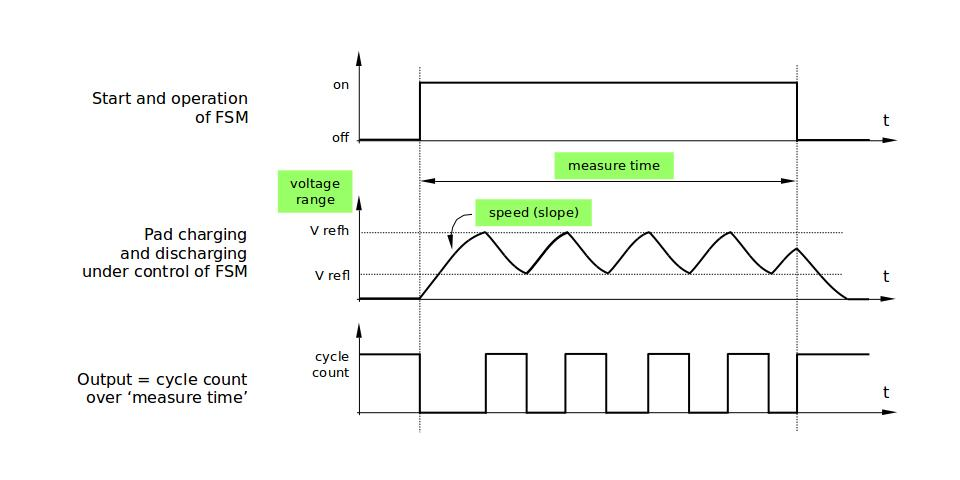
\includegraphics[width=0.8\textwidth]{images/FW/touch_parameters.jpg}
    \caption{ESP32 built-in touch sensor parameters}
    \label{fig:esp_touchparameters}
\end{figure}

\begin{figure}[ht]
    \centering
    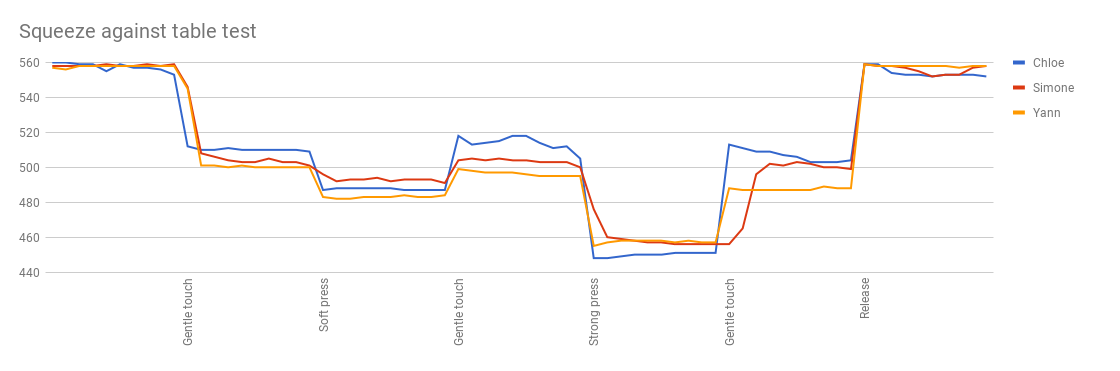
\includegraphics[width=\textwidth]{images/FW/capa_squeeze_table_multi.png}
    \caption{Test values for different touch/squeeze patterns with different users}
    \label{fig:esp_touchtest}
\end{figure}



\subsubsection{LEDs}\label{subsec:fw/Functions/LEDs}
    
\begin{figure}[H]
    \centering
    \subfloat[\label{fig:CHIC1}]{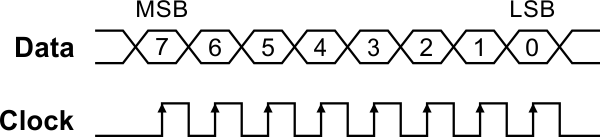
\includegraphics[width=0.6\textwidth]{images/FW/APA102.png}}\hfill
    \subfloat[\label{fig:APA102_1}] {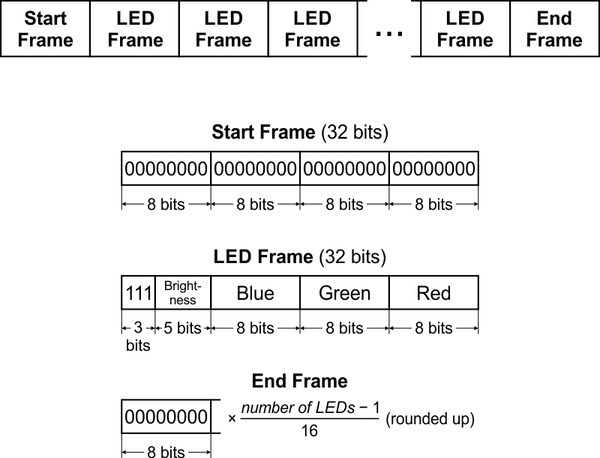
\includegraphics[width=0.8\textwidth]{images/FW/APA102_2.jpg}}\hfill
    \caption{APA102 communication protocol} 
    \label{fig:APA102}
\end{figure}   
   
\subsubsection{Capacitive touch sensors}
The Arduino environment does not allow easy tweaking of the capacitive touch sensors described in \ref{sec:capa_sens}. This can be done in C programs available from the ESP32 GitHub. We are still testing the parameters to find the right sensitivity and parameters, which depend on the shape and connections of the touch sensors.


    \subsubsection{Sound}
The Arduino Tone function and sound libraries have not been implemented yet for ESP32. In order to circumvent this problem, we use ESP32's LED PWN abilities to control our buzzer (described in Section \ref{subsubsec:hardware/esp32_capabilities}). With the PWM, the duty cycle and frequency can be set. We used a fixed duty cycle (which influences the loudness of sound) and used the frequency parameter to set up tones.


\lstinputlisting[style=Arduino, firstline=29, lastline=45]{code_snippets/arduino/Sound.ino}


\subsection{Next steps - functions to be implemented}
    \subsubsection{WiFi save Smartconfig in EEPROM}
    \subsubsection{Sleep functions}
    \subsubsection{Sound settings and implementing a proper loudspeaker}
    \subsubsection{Capacitive sensors calibration and touch/squeeze recognition}
    \subsubsection{Error checking}
    
    
    
